\section{Problems}

Here is a link to my code: \url{https://github.com/filipmellgren/QMM/tree/main/ps4}.

Thanks to Tom and Jonas for pointing out bugs in my code.

\begin{questions}
\question{Bequest questions}
\begin{solution}

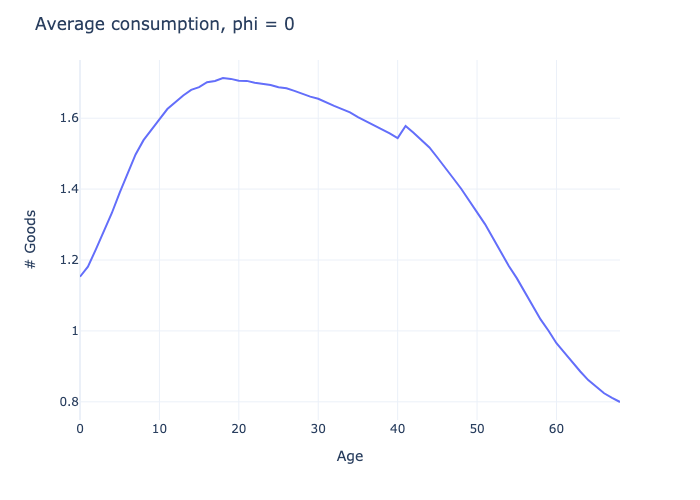
\includegraphics[scale=0.5]{figures/consumption_0_tax_15.png}

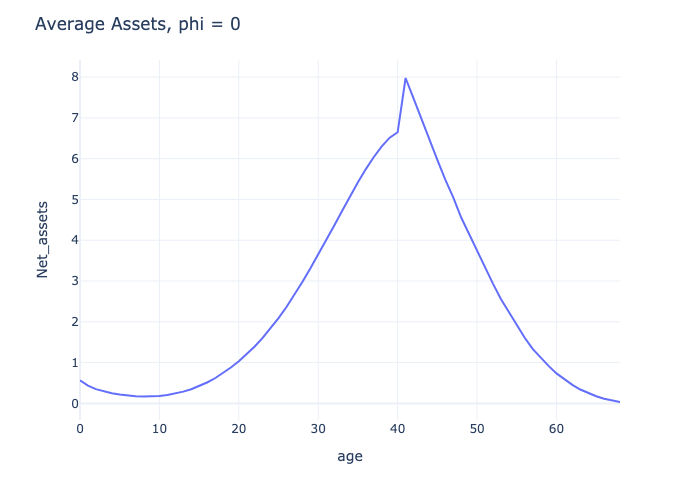
\includegraphics[scale=0.5]{figures/avg_assets_0_tax_15.png}

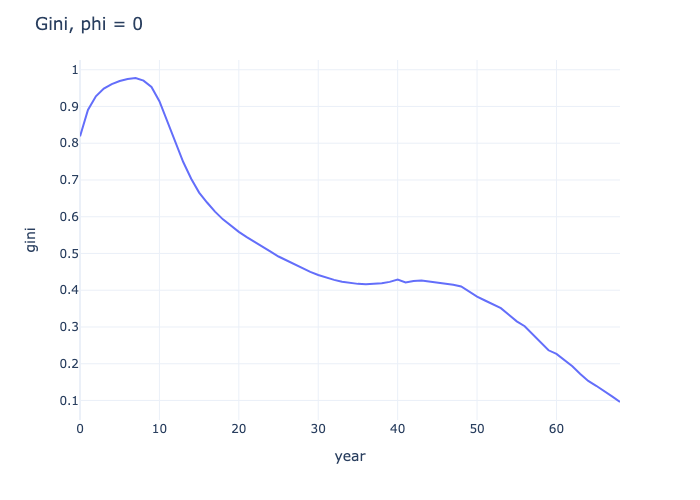
\includegraphics[scale=0.5]{figures/gini_0_tax_15.png}

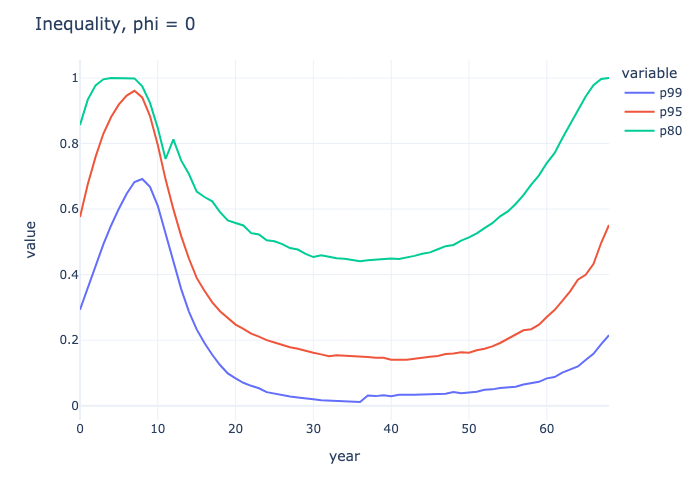
\includegraphics[scale=0.5]{figures/inequality_0_tax_15.png}

\end{solution}

\question{Life cycle paths of savings and consumption, and Lorenz curve}
\begin{solution}


\end{solution}

\question{Add bequest motive with $\phi_1 = -10$}
\begin{solution}
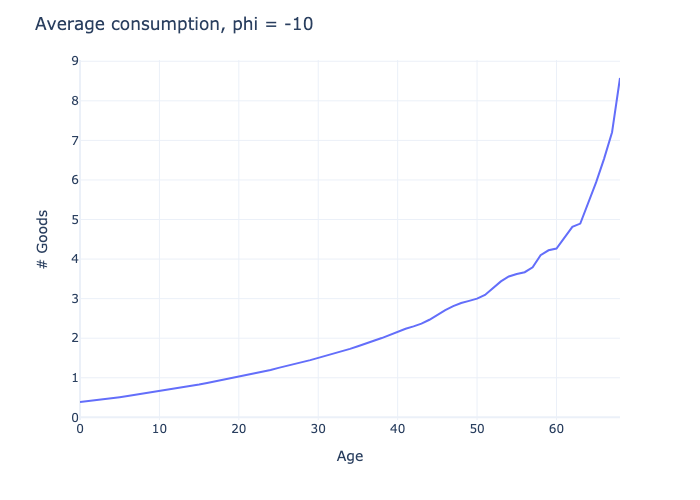
\includegraphics[scale=0.5]{figures/consumption_-10_tax_15.png}

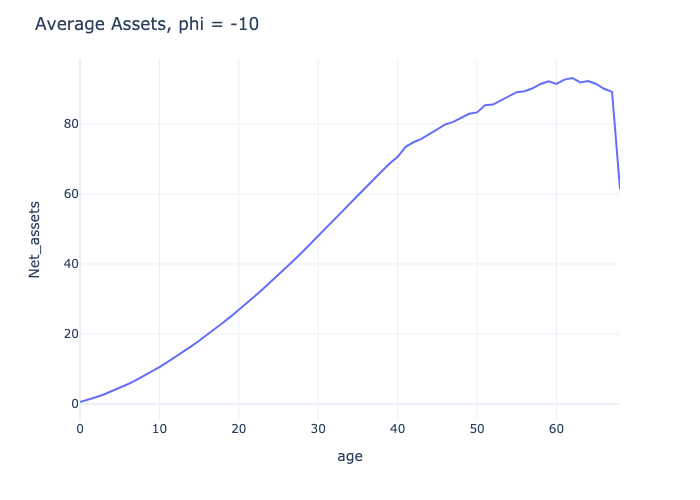
\includegraphics[scale=0.5]{figures/avg_assets_-10_tax_15.png}

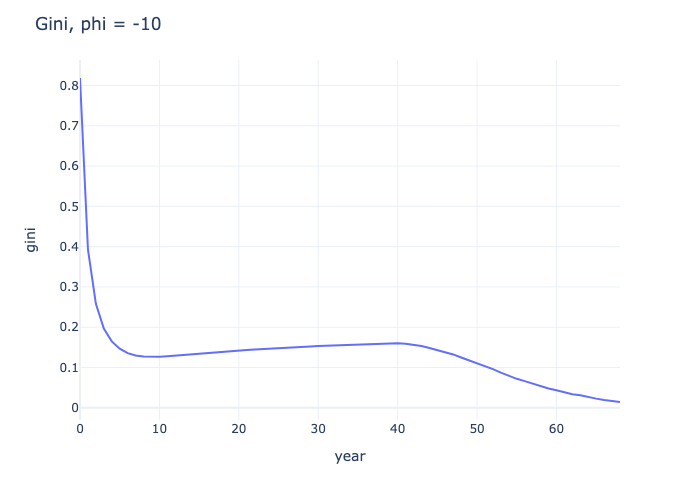
\includegraphics[scale=0.5]{figures/gini_-10_tax_15.png}

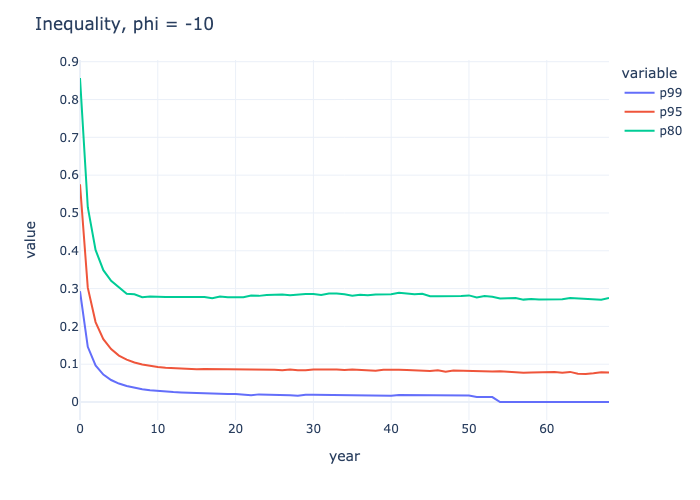
\includegraphics[scale=0.5]{figures/inequality_-10_tax_15.png}

The resulting graphs look wacky. Not sure why, but bequests seemingly much too high. Could be an issue with the terminal policy.
\end{solution}

\question{density comparison}
\begin{solution}
	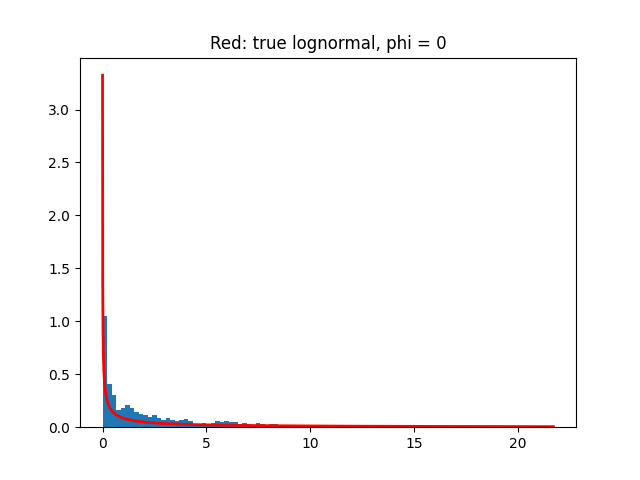
\includegraphics[scale=0.5]{figures/kdensity_0_tax_15.png}
\end{solution}

\question{Tax increase}
\begin{solution}
	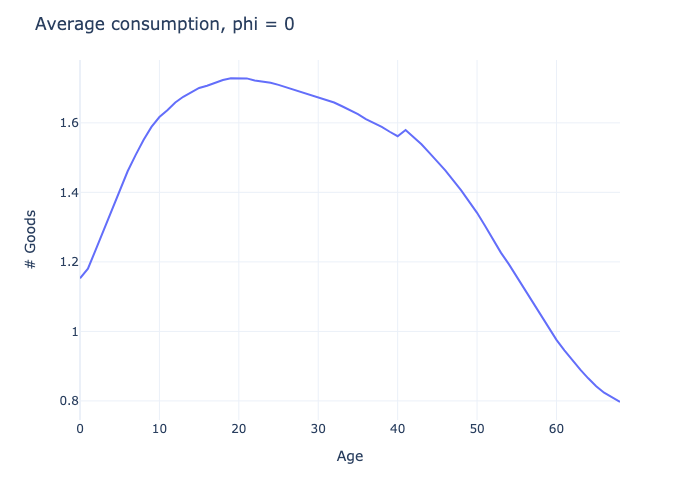
\includegraphics[scale=0.5]{figures/consumption_0_tax_30.png}

	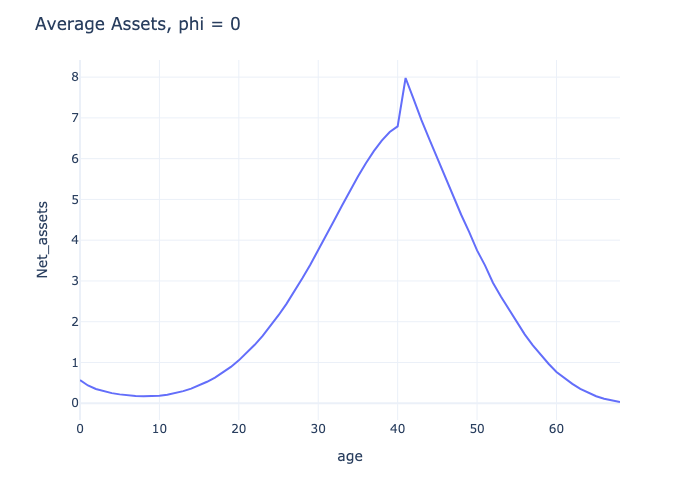
\includegraphics[scale=0.5]{figures/avg_assets_0_tax_30.png}

	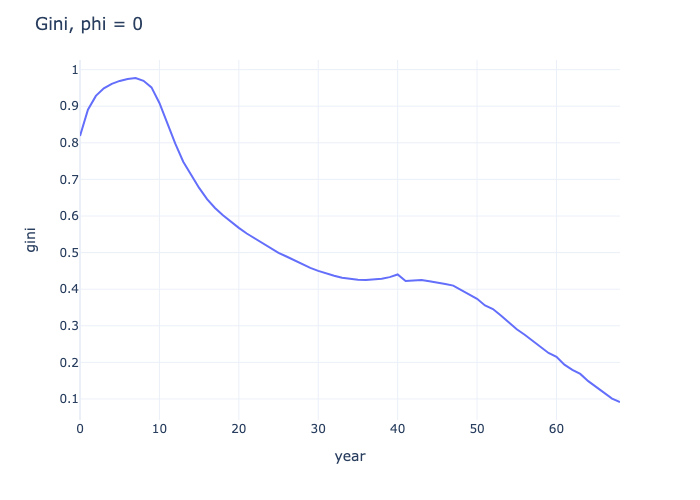
\includegraphics[scale=0.5]{figures/gini_0_tax_30.png}

	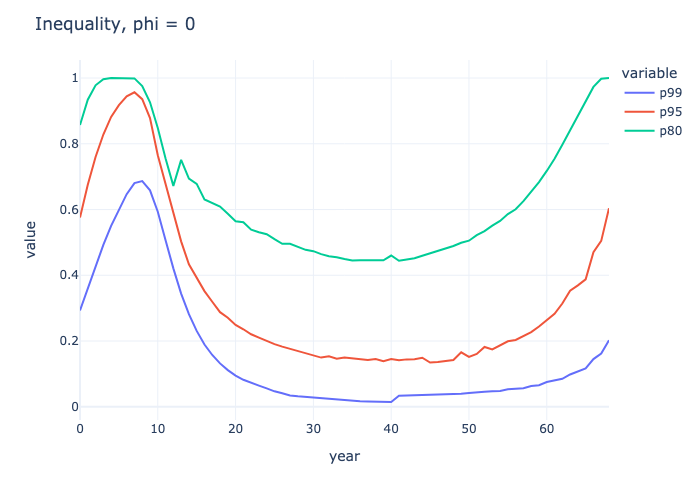
\includegraphics[scale=0.5]{figures/inequality_0_tax_30.png}
\end{solution}

No time to solve for the alternative tax policy.

\end{questions}


